\documentclass[journal]{IEEEtran}

% ------------------------------------------------------------------
\usepackage[utf8]{inputenc}
\usepackage{amsmath,amssymb,amsfonts}
\usepackage{graphicx}
\usepackage{booktabs}
\usepackage{multirow}
\usepackage{makecell}
\usepackage{array}
\usepackage{url}
\usepackage{xcolor}
\usepackage[hidelinks]{hyperref}
\usepackage{siunitx}
\usepackage{tikz}
\usepackage{pgfplots}
\pgfplotsset{compat=1.16}
\usetikzlibrary{arrows.meta,positioning,fit,backgrounds,calc}

\newcommand{\best}[1]{\textbf{#1}}

% ---- shared colors for figures ----
\definecolor{cenc}{RGB}{70,130,180}
\definecolor{cbottle}{RGB}{218,165,32}
\definecolor{cemb}{RGB}{60,179,113}
\definecolor{chead}{RGB}{205,92,92}
\definecolor{cprobe}{RGB}{120,120,120}
\definecolor{barA}{RGB}{70,130,180}
\definecolor{barB}{RGB}{60,179,113}
\definecolor{barC}{RGB}{205,92,92}
\definecolor{cdecoder}{RGB}{147,112,219}

\begin{document}

\title{DiffEEG: A Denoising-Diffusion Foundation Model\\
for Transferable EEG Representations Across\\
Seizure, Abnormality, Motor, and Sleep Tasks}

\author{Abdulkader~Helwan,~Lina~Abou-Abbas,~Hussein~El~Amouri,~Belkacem~Chikhaoui,~and~Khadidja~Henni
\thanks{A. Helwan, L. Abou-Abbas, and H. El Amouri are with the Department of Electrical and Computer Engineering, Lebanese American University, Byblos, Lebanon.}
\thanks{B. Chikhaoui and K. Henni are with the Institute of Applied Artificial Intelligence, TÉLUQ University, Montréal, Canada.}
\thanks{Corresponding author: A. Helwan (e-mail: abdulkader.helwan90@gmail.com).}}

\markboth{Preprint --- EEG Foundation Models}{Helwan \MakeLowercase{et al.}: DiffEEG: A Denoising-Diffusion Foundation Model for Transferable EEG Representations}

\maketitle

% ==================================================================
\begin{abstract}
% ==================================================================
Electroencephalography (EEG) foundation models aim to learn task- and
subject-invariant representations that transfer to many downstream problems.
Most existing models are pretrained with masked or contrastive objectives and
are evaluated with full fine-tuning on benchmarks whose preprocessing matches
pretraining. We present \textsc{DiffEEG}, a \num{40.7}M-parameter
denoising-diffusion model that learns generic EEG representations by
reconstructing clean signals from noisy inputs, and that is used as a
frozen feature extractor for downstream tasks. Representations are
obtained by probing the diffusion denoiser at five noise levels and pooling its
hierarchical encoder activations into a \num{4800}-dimensional descriptor. A
lightweight channel-harmonization front end projects any electrode montage onto
a canonical 22-channel frame, allowing a single fixed-input model to process
datasets recorded with different hardware. We adapt the embedding with a linear
probe, partial fine-tuning, and a reinforcement-learning (RL) head that directly
optimizes macro-F1. Across seven datasets spanning four task families---seizure
detection (TUSZ, Siena, Bonn), EEG abnormality and event classification (TUAB,
TUEV), motor imagery (EEGMMIDB), and sleep staging (Sleep-EDFx)---the diffusion
embedding transfers effectively: it reaches \num{0.993} ROC-AUC on Bonn seizure
detection, \num{94.0}\% accuracy on patient-wise TUSZ seizure detection,
\num{0.878} ROC-AUC (\num{79.3}\% accuracy) on TUAB abnormality detection, and
above-chance accuracy on tasks the backbone never saw during pretraining,
including motor imagery (\num{61.5}\%) and six-class sleep staging
(\num{53.9}\%). The RL head is
particularly effective under extreme class imbalance, improving minority-class
precision by up to eight-fold on the \num{0.64}\%-prevalence Siena corpus---the
operating regime of continuous clinical monitoring. Compared with recent
foundation models on accuracy, macro/weighted-F1, and ROC-AUC, \textsc{DiffEEG}
is competitive on clinical abnormality detection while offering broad, low-cost
transfer from a single generative backbone. To support clinical
interpretability, we analyze the learned representation: t-SNE of the frozen
embedding shows that pretraining alone organizes clinically meaningful event
categories, and gradient-based saliency localizes the scalp regions and time
segments that drive epileptiform decisions, in agreement with known
electrophysiology.
\end{abstract}

\begin{IEEEkeywords}
EEG, foundation model, denoising diffusion, representation learning, transfer
learning, reinforcement learning, seizure detection, sleep staging.
\end{IEEEkeywords}

% ==================================================================
\section{Introduction}
% ==================================================================
\IEEEPARstart{E}{lectroencephalography} (EEG) is the primary non-invasive tool
for diagnosing epilepsy and screening for cerebral abnormality, and it underpins
a wide range of clinical and brain--computer interface (BCI) applications,
including seizure detection, abnormality screening, sleep staging, and motor
decoding~\cite{obeid2016tuh,roy2019dl}. Manual EEG review is labor-intensive,
requires scarce sub-specialist expertise, and suffers from substantial
inter-rater variability; automated decision support could therefore materially
improve the consistency and reach of neurological care. Yet clinical EEG poses
challenges that generic deep learning handles poorly: pathological events
(seizures, epileptiform discharges) are rare, occupying a small fraction
of continuous recordings, so models optimized for accuracy collapse onto the
majority ``normal'' class; and models trained for one task, montage, or
institution rarely transfer to another, while the volume of expert annotation
required to retrain them is a persistent barrier. These constraints have
motivated EEG foundation models (FMs): networks pretrained self-supervised
on large unlabeled corpora and adapted to specific downstream
tasks~\cite{yang2024biot,jiang2024labram,wang2024cbramod,wang2024eegpt}.

Two characteristics dominate the current FM literature. First, nearly all models
are pretrained with masked or contrastive objectives adapted from
language and vision. Second, they are usually evaluated by full
fine-tuning on benchmarks whose channel montage, sampling rate, and window
length match those used during pretraining. As a result, it is not well
understood whether a generative pretraining objective produces
representations as transferable as masked prediction, nor how well a pretrained
EEG model behaves as a frozen embedding that must adapt to genuinely
different montages and tasks with little fine-tuning---the regime that matters
most for rapid BCI calibration and low-label clinical deployment.

This paper studies both questions using \textsc{DiffEEG}, a denoising-diffusion
model that is pretrained purely to reconstruct clean EEG and then used as a
general-purpose feature extractor. Rather than training a task-specific network
end-to-end, we probe the frozen diffusion denoiser at several noise levels and
pool its multi-scale encoder activations into a single descriptor. Because the
backbone accepts a fixed 22-channel input, we introduce a channel-harmonization
front end that maps any montage onto the model's canonical frame, enabling a
single frozen model to be exercised on datasets with $1$--$64$ native channels
and $100$--$512$\,Hz native sampling rates. The embedding is then adapted with a
head-only classifier, partial fine-tuning, or a reinforcement-learning head that
directly optimizes macro-F1.

The contributions of this work are:
\begin{enumerate}
  \item A multi-timestep diffusion-probing embedding that turns a
  generative EEG denoiser into a compact \num{4800}-dimensional feature
  extractor supporting head-only classification.
  \item A channel-harmonization pipeline that projects arbitrary
  montages onto a canonical 22-channel frame, allowing a fixed-input model to be
  applied to heterogeneous datasets.
  \item A broad transfer evaluation across seven datasets and four task
  families, with head-only adaptation, fine-tuning, and reinforcement-learning
  adaptation, and a direct comparison against recent foundation models on
  accuracy, macro/weighted-F1, ROC-AUC, and AUC-PR.
  \item An interpretability analysis tailored to clinical use:
  embedding-space visualization showing that the pretrained representation
  organizes clinically meaningful event categories, and gradient-based saliency
  that localizes the electrodes and time segments driving epileptiform
  decisions.
\end{enumerate}

% ==================================================================
\section{Related Work}
% ==================================================================
\subsection{EEG foundation models}
BIOT~\cite{yang2024biot} tokenizes biosignals into fixed-length segments to
learn across datasets with mismatched channels. LaBraM~\cite{jiang2024labram}
introduces a neural tokenizer with vector-quantized spectral prediction and
scales to hundreds of millions of parameters.
CBraMod~\cite{wang2024cbramod} uses a criss-cross transformer that models
temporal and spatial dependencies separately and popularized linear-probing
evaluation. EEGPT~\cite{wang2024eegpt} aligns spatio-temporal representations
with a dual self-supervised objective. More recent models target montage
generalization: \textsc{NeurIPT}~\cite{fang2025neuript} adds 3D electrode
coordinate encodings, amplitude-aware masked pretraining, and a progressive
mixture-of-experts; \textsc{REVE}~\cite{elouahidi2025reve} scales masked
autoencoding to \num{60000} hours from $92$ datasets and \num{25000} subjects
with a 4D positional encoding that natively accepts arbitrary montages. In the
clinical seizure domain, \textsc{BioSerenity-E1}~\cite{bettinardi2025bioserenity}
combines spectral tokenization with masked prediction and reports strong AUROC
on the TUH Seizure corpus.

\subsection{Diffusion models for representation learning}
Denoising diffusion probabilistic models~\cite{ho2020ddpm,nichol2021improved}
learn to invert a gradual noising process and are the dominant paradigm for
generative modeling. Beyond synthesis, the intermediate activations of a trained
denoiser encode semantically meaningful features whose abstraction level varies
with the noise level. \textsc{DiffEEG}~\cite{helwan2025diffeeg} first applied
this idea to seizure detection. The present work differs in two ways: it studies
the model as a general embedding rather than a seizure classifier, and it
evaluates transfer across four task families under montage and task shift rather
than a single in-domain benchmark.

% ==================================================================
\section{Methods}
% ==================================================================
\subsection{Diffusion backbone}
\textsc{DiffEEG} is a conditional 1D~U-Net trained to reverse a cosine-schedule
Gaussian noising process over $T=1000$ timesteps~\cite{ho2020ddpm,nichol2021improved}.
Given a clean segment $x_0\in\mathbb{R}^{C\times L}$ with $C=22$ channels and
$L=1280$ samples (\SI{5}{\second} at \SI{256}{\hertz}), the forward process adds
noise as
\begin{equation}
x_t=\sqrt{\bar\alpha_t}\,x_0+\sqrt{1-\bar\alpha_t}\,\epsilon,\quad
\epsilon\sim\mathcal N(0,\mathbf I),
\end{equation}
and the network $\epsilon_\theta(x_t,t)$ is trained with the noise-prediction
loss $\mathcal L=\mathbb E_{x_0,\epsilon,t}\lVert\epsilon-\epsilon_\theta(x_t,t)\rVert^2$.
The backbone uses base width $m=64$, channel multipliers $[1,2,4,8]$ (encoder
feature widths $\{64,128,256,512\}$), three residual blocks per level with
feature-wise linear modulation (FiLM)~\cite{perez2018film} conditioning on the
timestep, and multi-head self-attention at the deeper encoder levels and the
bottleneck. The full model has \num{40679574} parameters. The encoder--decoder
is trained end-to-end during pretraining; for downstream use the decoder is
discarded and only the encoder is retained as a feature extractor.

\subsection{Network architecture in detail}
\label{sec:arch}
Figure~\ref{fig:archdetail} details the backbone used throughout this work
(the training configuration referred to as V2, with base width $m=64$,
channel multipliers $[1,2,4,8]$, three residual blocks per encoder level, and
time embedding dimension 768). The network takes the noisy input
$x_t\in\mathbb{R}^{22\times1280}$ together with the scalar timestep $t$ and
outputs the predicted noise $\hat\epsilon\in\mathbb{R}^{22\times1280}$.

The timestep is first mapped to a 768-dimensional embedding by a sinusoidal
position encoding followed by a two-layer MLP ($768\to1536\to768$, SiLU
activation); this embedding conditions every residual block in the network.
A $3\times3$ convolution (\texttt{init\_conv}) projects the 22 input channels
to the base width of 64.

The encoder has four resolution levels with channel widths
$\{64,128,256,512\}$. Each level applies three residual blocks at a fixed
channel count and temporal length, followed by a strided ($\mathrm{stride}=2$)
$3\times3$ convolution that halves the sequence length; three such
downsampling steps take the sequence from 1280 samples to 160 samples by the
end of the encoder. Self-attention (8 heads) is applied only in the last
residual block of the two deepest encoder levels (256 and 512 channels),
leaving the shallow, high-resolution levels purely convolutional for
efficiency. The bottleneck operates at 160 samples and 512 channels with
three residual blocks, all with self-attention.

The decoder mirrors the encoder in reverse, with four levels returning the
channel width to $\{512,256,128,64\}$ and the sequence length from 160 back
to 1280 samples via three upsampling steps (linear interpolation by a factor
of 2 followed by a $3\times3$ convolution). Because the additive skip
connection is folded into the first residual block at each decoder level, the
decoder uses one more residual block per level than the encoder, four instead
of three. Self-attention is applied in the first residual block of the two
decoder levels closest to the bottleneck (512 and 256 channels). Each decoder
level receives an additive skip connection from the output of the
corresponding encoder level (resized by linear interpolation if the temporal
lengths differ after non-integer downsampling), which is added to the input
of that level's first residual block, in the same spirit as the original
U-Net~\cite{ronneberger2015unet}. A final instance normalization, a
$1\times1$ convolution back to 64 channels, and a $3\times3$ convolution to
22 channels produce the predicted noise.

Every residual block (Fig.~\ref{fig:resblock}) follows the same pattern:
instance normalization, SiLU, a $3\times3$ convolution, feature-wise linear
modulation (FiLM)~\cite{perez2018film} that applies a per-channel scale and
shift derived from the timestep embedding, a second
normalization--SiLU--dropout--convolution pair, an optional multi-head
self-attention over the temporal axis, and a residual connection (with a
$1\times1$ projection when the channel count changes). In total the network
contains 31 residual blocks (12 in the encoder, 3 in the bottleneck, and 16
in the decoder), of which 7 include the attention module, for
\num{40679574} parameters overall.

\begin{figure*}[t]
\centering
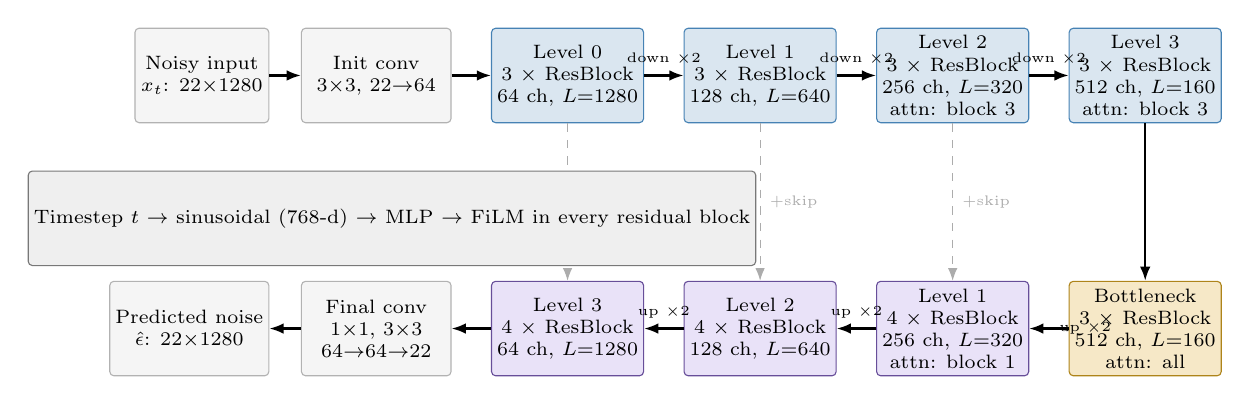
\begin{tikzpicture}[
  font=\scriptsize,
  box/.style={draw, rounded corners=1.5pt, minimum height=12mm, minimum width=19mm, align=center, inner sep=2pt},
  enc/.style={box, fill=cenc!20, draw=cenc},
  dec/.style={box, fill=cdecoder!20, draw=cdecoder!70!black},
  bott/.style={box, fill=cbottle!25, draw=cbottle!80!black},
  io/.style={box, fill=gray!8, draw=gray!60, minimum width=17mm},
  ar/.style={-{Latex[length=1.8mm]}, thick},
  skip/.style={-{Latex[length=1.6mm]}, dashed, gray!65, thin},
]
% ---- top row: encoder ----
\node[io] (in) {Noisy input\\$x_t$: 22$\times$1280};
\node[box, fill=gray!8, draw=gray!60, right=4mm of in] (init) {Init conv\\$3{\times}3$, 22$\to$64};
\node[enc, right=5mm of init] (l0) {Level 0\\3 $\times$ ResBlock\\64 ch, $L{=}1280$};
\node[enc, right=5mm of l0] (l1) {Level 1\\3 $\times$ ResBlock\\128 ch, $L{=}640$};
\node[enc, right=5mm of l1] (l2) {Level 2\\3 $\times$ ResBlock\\256 ch, $L{=}320$\\attn: block 3};
\node[enc, right=5mm of l2] (l3) {Level 3\\3 $\times$ ResBlock\\512 ch, $L{=}160$\\attn: block 3};
\draw[ar] (in) -- (init);
\draw[ar] (init) -- (l0);
\draw[ar] (l0) -- node[above,font=\tiny]{down $\times2$} (l1);
\draw[ar] (l1) -- node[above,font=\tiny]{down $\times2$} (l2);
\draw[ar] (l2) -- node[above,font=\tiny]{down $\times2$} (l3);

% ---- bottleneck, bottom-right ----
\node[bott, below=20mm of l3] (bn) {Bottleneck\\3 $\times$ ResBlock\\512 ch, $L{=}160$\\attn: all};
\draw[ar] (l3) -- (bn);

% ---- bottom row: decoder, columns aligned under l2,l1,l0 ----
\node[dec, below=20mm of l2] (d1) {Level 1\\4 $\times$ ResBlock\\256 ch, $L{=}320$\\attn: block 1};
\node[dec, below=20mm of l1] (d2) {Level 2\\4 $\times$ ResBlock\\128 ch, $L{=}640$};
\node[dec, below=20mm of l0] (d3) {Level 3\\4 $\times$ ResBlock\\64 ch, $L{=}1280$};
\node[box, fill=gray!8, draw=gray!60, left=5mm of d3] (final) {Final conv\\$1{\times}1$, $3{\times}3$\\64$\to$64$\to$22};
\node[io, left=4mm of final] (out) {Predicted noise\\$\hat\epsilon$: 22$\times$1280};
\draw[ar] (bn) -- node[right,font=\tiny]{up $\times2$} (d1);
\draw[ar] (d1) -- node[above,font=\tiny]{up $\times2$} (d2);
\draw[ar] (d2) -- node[above,font=\tiny]{up $\times2$} (d3);
\draw[ar] (d3) -- (final);
\draw[ar] (final) -- (out);

% ---- skip connections (additive) ----
\draw[skip] (l0) -- (d3) node[midway,right,font=\tiny]{+skip};
\draw[skip] (l1) -- (d2) node[midway,right,font=\tiny]{+skip};
\draw[skip] (l2) -- (d1) node[midway,right,font=\tiny]{+skip};

% ---- time embedding ----
\node[box, fill=cprobe!12, draw=cprobe, below=6mm of init, xshift=2mm, minimum width=30mm]
  (temb) {Timestep $t$ $\to$ sinusoidal (768-d) $\to$ MLP $\to$ FiLM in every residual block};
\end{tikzpicture}
\caption{Detailed architecture of the DiffEEG 1D~U-Net (V2 configuration).
Top row: encoder, four levels with channel widths 64, 128, 256, 512 and three
residual blocks per level; strided convolutions halve the sequence length
between levels. Bottom row: decoder, mirroring the encoder with one extra
residual block per level (four) to absorb the additive skip connection, and
transposed-resolution upsampling. Dashed arrows denote the additive skip
connections from each encoder level into the corresponding decoder level.
Self-attention (8 heads) is used only in the deepest two encoder levels, the
full bottleneck, and the two decoder levels nearest the bottleneck.}
\label{fig:archdetail}
\end{figure*}

\begin{figure}[t]
\centering
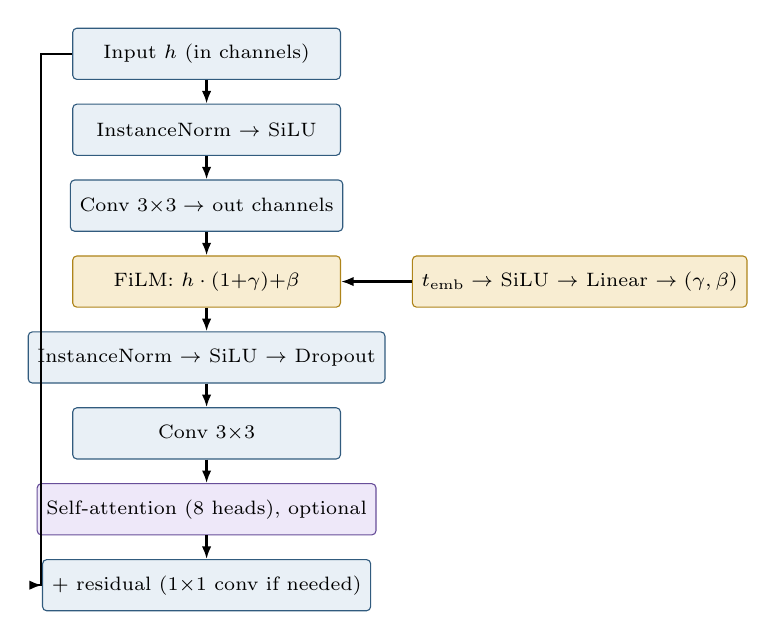
\begin{tikzpicture}[
  font=\scriptsize,
  rbstep/.style={draw, rounded corners=1.5pt, minimum height=6.5mm, minimum width=34mm, align=center, fill=cenc!12, draw=cenc!70!black},
  filmstep/.style={rbstep, fill=cbottle!20, draw=cbottle!80!black},
  attnstep/.style={rbstep, fill=cdecoder!16, draw=cdecoder!70!black},
  ar/.style={-{Latex[length=1.6mm]}, thick},
]
\node[rbstep] (in) {Input $h$ (in channels)};
\node[rbstep, below=3mm of in] (n1) {InstanceNorm $\to$ SiLU};
\node[rbstep, below=3mm of n1] (c1) {Conv $3{\times}3\to$ out channels};
\node[filmstep, below=3mm of c1] (film) {FiLM: $h\cdot(1{+}\gamma){+}\beta$};
\node[rbstep, below=3mm of film] (n2) {InstanceNorm $\to$ SiLU $\to$ Dropout};
\node[rbstep, below=3mm of n2] (c2) {Conv $3{\times}3$};
\node[attnstep, below=3mm of c2] (attn) {Self-attention (8 heads), optional};
\node[rbstep, below=3mm of attn] (out) {$+$ residual ($1{\times}1$ conv if needed)};
\node[filmstep, right=9mm of film, minimum width=26mm] (temb) {$t_{\mathrm{emb}}\to$ SiLU $\to$ Linear $\to(\gamma,\beta)$};
\draw[ar] (in) -- (n1); \draw[ar] (n1) -- (c1); \draw[ar] (c1) -- (film);
\draw[ar] (film) -- (n2); \draw[ar] (n2) -- (c2); \draw[ar] (c2) -- (attn);
\draw[ar] (attn) -- (out); \draw[ar] (temb) -- (film);
\draw[ar] (in.west) -- ++(-4mm,0) |- (out.west);
\end{tikzpicture}
\caption{Internal structure of a single residual block. The timestep
embedding $t_{\mathrm{emb}}$ is projected to a per-channel scale $\gamma$ and
shift $\beta$ (FiLM) that condition the block on the diffusion noise level.
The self-attention step is present only in 7 of the 31 blocks in the network
(Fig.~\ref{fig:archdetail}).}
\label{fig:resblock}
\end{figure}

\subsection{Multi-timestep diffusion-probing embedding}
\label{sec:embedding}
To turn the denoiser into a feature extractor we probe the encoder at a fixed
set of diffusion timesteps
\begin{equation}
\mathcal T=\{50,250,500,750,950\}
\end{equation}
that uniformly span the noise schedule. Low-noise probes preserve fine temporal
detail (e.g.\ spikes, spindles) while high-noise probes capture coarse
morphology. For an input segment $x$, we form the noised input $x_t$ at each
$t\in\mathcal T$, run the encoder, and apply global adaptive average pooling to
each of the four encoder levels $\ell\in\{1,2,3,4\}$:
\begin{equation}
f^{(t)}_\ell=\frac{1}{L_\ell}\sum_{i=1}^{L_\ell}h^{(t)}_{\ell,i}\in\mathbb R^{d_\ell},
\quad d_\ell\in\{64,128,256,512\}.
\end{equation}
Concatenating across all levels and timesteps yields the embedding
\begin{equation}
z=\bigoplus_{t\in\mathcal T}\bigoplus_{\ell=1}^{4}f^{(t)}_\ell\in\mathbb R^{D},
\quad
D=|\mathcal T|\!\times\!\!\sum_\ell d_\ell = 5\times960 = 4800 .
\end{equation}
This \num{4800}-dimensional vector is the fixed EEG descriptor used by all
downstream tasks. Because it is computed from a frozen backbone with
deterministic noising seeds, it is precomputed and cached once per dataset.
Fig.~\ref{fig:arch} summarizes the full pipeline.

\begin{figure*}[t]
\centering
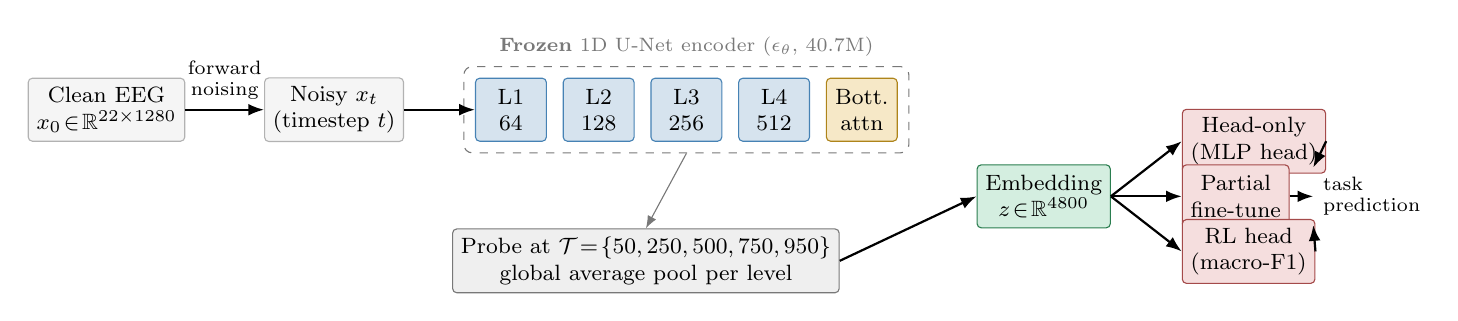
\begin{tikzpicture}[
  font=\footnotesize,
  box/.style={draw, rounded corners=1.5pt, minimum height=8mm, align=center, inner sep=3pt},
  enc/.style={box, fill=cenc!22, draw=cenc, minimum width=9mm},
  bott/.style={box, fill=cbottle!25, draw=cbottle!80!black, minimum width=9mm},
  emb/.style={box, fill=cemb!22, draw=cemb!70!black},
  head/.style={box, fill=chead!20, draw=chead!80!black},
  io/.style={box, fill=gray!8, draw=gray!60},
  ar/.style={-{Latex[length=2mm]}, thick},
  arp/.style={-{Latex[length=1.6mm]}, cprobe},
]
% --- pretraining strip (top) ---
\node[io] (x0) {Clean EEG\\$x_0\!\in\!\mathbb{R}^{22\times1280}$};
\node[io, right=10mm of x0] (xt) {Noisy $x_t$\\(timestep $t$)};
\draw[ar] (x0) -- node[above,align=center]{\scriptsize forward\\[-2pt]\scriptsize noising} (xt);

% --- frozen encoder ---
\node[enc, right=9mm of xt] (l1) {L1\\64};
\node[enc, right=2mm of l1] (l2) {L2\\128};
\node[enc, right=2mm of l2] (l3) {L3\\256};
\node[enc, right=2mm of l3] (l4) {L4\\512};
\node[bott, right=2mm of l4] (bn) {Bott.\\attn};
\draw[ar] (xt) -- (l1);
\begin{scope}[on background layer]
  \node[draw=cprobe, dashed, rounded corners=3pt, fit=(l1)(bn),
        inner sep=4pt, label={[cprobe]above:\scriptsize \textbf{Frozen} 1D~U-Net encoder ($\epsilon_\theta$, 40.7M)}] (encbox) {};
\end{scope}

% --- probing / pooling ---
\node[box, fill=cprobe!12, draw=cprobe, below=11mm of l2.south, xshift=6mm, align=center] (gap)
  {Probe at $\mathcal{T}\!=\!\{50,250,500,750,950\}$\\global average pool per level};
\draw[arp] (encbox.south) -- (gap.north);

% --- embedding ---
\node[emb, right=10mm of bn, yshift=-11mm] (z) {Embedding\\$z\!\in\!\mathbb{R}^{4800}$};
\draw[ar] (gap.east) -- (z.west);

% --- heads ---
\node[head, right=9mm of z, yshift=7mm] (lp) {Head-only\\(MLP head)};
\node[head, right=9mm of z] (ft) {Partial\\fine-tune};
\node[head, right=9mm of z, yshift=-7mm] (rl) {RL head\\(macro-F1)};
\draw[ar] (z.east) -- (lp.west);
\draw[ar] (z.east) -- (ft.west);
\draw[ar] (z.east) -- (rl.west);
\node[right=3mm of ft, align=left] (out) {\scriptsize task\\[-2pt]\scriptsize prediction};
\draw[ar] (lp.east) -- (out.north west);
\draw[ar] (ft.east) -- (out.west);
\draw[ar] (rl.east) -- (out.south west);
\end{tikzpicture}
\caption{DiffEEG pipeline. A 1D~U-Net is pretrained to denoise EEG (generative
objective). For downstream use the frozen encoder is probed at five diffusion
timesteps; per-level global average pooling and concatenation yield a
\num{4800}-dimensional embedding, which is adapted by a head-only classifier,
partial fine-tuning, or a reinforcement-learning head.}
\label{fig:arch}
\end{figure*}

\subsection{Head-only}
\label{subsec:headonly}
The default adaptation is head-only training: the backbone is frozen and a
two-layer multilayer perceptron (MLP) classifier with batch normalization, GELU
activation, and dropout is trained on the cached embedding $z$. Training uses
weighted cross-entropy with inverse-frequency class weights
$w_k = N/(K\,n_k)$, where $N$ is the total number of samples, $K$ the number of
classes, and $n_k$ the count of class $k$, to counter class imbalance. Head-only
training isolates the quality of the pretrained representation, since only the
head is optimized.
\subsection{Embedding-only evaluation}
\label{subsec:embonly}
A natural concern is that the 2-layer MLP head is itself a small trainable classifier, so its performance mixes two confounded signals: (i) the quality of the embedding, and (ii) the additional capacity of the head. To isolate (i), we report a strictly non-parametric evaluation of the embedding using k-nearest-neighbor classification on the 4800-d embedding space.
We adopt k-NN rather than the more common single-layer logistic-regression classifier because k-NN is bounded above by the best parametric probe yet makes no assumption about the form of the decision boundary. In our setting this is the more useful endpoint: it directly measures the local class consistency of the embedding space, which is the property a downstream user of the embedding most cares about.
When additional capacity is warranted, we unfreeze part or all of the backbone.
A gentle differential learning rate is used: the head is trained at
$\eta_{\mathrm{head}}=5\times10^{-4}$ while unfrozen backbone layers use
$\eta_{\mathrm{backbone}}=0.01\,\eta_{\mathrm{head}}$, which avoids the
optimization collapse that a single aggressive learning rate causes on small
downstream datasets. Unfreezing is controlled from \texttt{last\_level} (only
the deepest encoder level) to \texttt{all} (the full encoder and bottleneck).

\subsection{Reinforcement-learning decision head}
For imbalanced tasks, per-sample cross-entropy tends to favor the majority
class. We therefore add a reinforcement-learning (RL) decision head that
directly optimizes the target evaluation metric. A policy network
$\pi_\phi:\mathbb R^{D}\!\to\!\mathbb R^{K}$ produces class logits; during
training we sample predictions from the resulting Categorical distribution and
receive the batch macro-F1 as the reward $R$. Using the REINFORCE
estimator~\cite{he2022rl} with an exponential-moving-average baseline $b$ for
variance reduction, the policy-gradient loss is
\begin{equation}
\mathcal L_{\mathrm{PG}}=-(R-b)\,\frac{1}{N_b}\sum_{i=1}^{N_b}\log \pi_\phi(\hat y_i\mid z_i),
\end{equation}
and the total objective combines it with weighted cross-entropy,
\begin{equation}
\mathcal L=\mathcal L_{\mathrm{CE}}+\lambda\,\mathcal L_{\mathrm{PG}},\qquad \lambda=0.1 .
\end{equation}
The macro-F1 reward makes the head sensitive to rare classes and generalizes to
any number of classes, so the same mechanism is used for binary and multi-class
tasks.

\subsection{Channel harmonization}
\label{sec:channels}
The backbone accepts exactly $22$ channels in a fixed referential order
(FP1, FP2, F3, F4, C3, C4, P3, P4, O1, O2, F7, F8, T3, T4, T5, T6, A1, A2, FZ,
CZ, PZ, ROC). For each recording we (i)~canonicalize electrode names,
(ii)~map them onto the 22-slot frame by exact match and then a curated alias
table (e.g.\ $\text{T7}\!\to\!\text{T3}$, $\text{P7}\!\to\!\text{T5}$,
$\text{TP9}\!\to\!\text{A1}$; for bipolar-only montages
$\text{Fpz--Cz}\!\to\!\text{FZ}$, $\text{Pz--Oz}\!\to\!\text{PZ}$),
(iii)~zero-fill any target channel with no matching electrode, and
(iv)~resample the session to \SI{256}{\hertz} before windowing. Unmatched
channels are zero-filled rather than interpolated, so the model never receives
fabricated signal. The number of real channels a dataset contributes is
therefore an explicit quantity (Table~\ref{tab:datasets}).

% ==================================================================
\section{Experiments and Implementation}
% ==================================================================
\subsection{Data processing}
All datasets are converted to the model's input format---$22$ channels,
\SI{256}{\hertz}, \SI{5}{\second} ($1280$-sample) windows---using the
harmonization pipeline of Section~\ref{sec:channels}. Table~\ref{tab:datasets}
summarizes each dataset's native characteristics and the outcome of
harmonization. For datasets whose raw amplitude scale differs from the
pretraining convention (e.g.\ Siena, recorded in volts), we compute
dataset-specific normalization statistics; for datasets without global
statistics we apply per-window z-scoring. TUEV carries short discrete event
annotations rather than continuous labels, so windows are extracted centered on
each merged event rather than on a fixed grid.

\begin{table*}[t]
\centering
\caption{Datasets, native acquisition characteristics, and the result of
harmonization onto the canonical 22-channel frame.}
\label{tab:datasets}
\small
\begin{tabular}{@{}llrrrrl@{}}
\toprule
Dataset & Task family & \makecell[r]{Native\\chans} & \makecell[r]{Native\\rate} &
\makecell[r]{Real ch.\\/ 22} & \makecell[r]{Zero-\\filled} & Split \\
\midrule
TUSZ       & Seizure detection            & 29 & \SI{256}{\hertz} & 22 & 0  & patient-wise (official eval) \\
Siena      & Seizure detection            & 45 & \SI{512}{\hertz} & 19 & 3  & patient-wise (11/3) \\
Bonn       & Seizure detection            & 1  & \SI{173.6}{\hertz} & 1 & 21 & record-wise \\
TUAB       & Abnormality detection        & 36 & \SI{250}{\hertz} & 22 & 0  & official train/eval \\
TUEV       & Event classification         & 27 & \SI{250}{\hertz} & 22 & 0  & official train/eval \\
EEGMMIDB   & Motor imagery                & 64 & \SI{160}{\hertz} & 19 & 3  & subject-wise \\
Sleep-EDFx & Sleep staging                & 2  & \SI{100}{\hertz} & 2  & 20 & subject-wise \\
\bottomrule
\end{tabular}
\end{table*}

\subsection{Pretraining}
\label{subsec:pretraining}
The diffusion backbone is pretrained, fully self-supervised, on
$\approx\!\num{1.45}$M unlabeled five-second segments of clinical EEG drawn from
three corpora: the non-seizure segments of the Temple University Hospital
Seizure Corpus (TUSZ) and of CHB-MIT, together with the normal recordings of the
Temple University Hospital Abnormal Corpus (TUAB). Segments are extracted with
$30\%$ overlap, notch-filtered at \SI{50}{\hertz}, band-pass filtered between
\SI{1}{} and \SI{75}{\hertz} with a zero-phase Butterworth filter, and
channel-wise normalized. Training minimizes the noise-prediction loss with a
cosine variance schedule ($T=1000$) using AdamW; no labels are used.

We note one caveat that affects interpretation of the TUAB result: because the
\emph{normal} recordings of TUAB---including its official held-out test-normal
split---are part of this pretraining corpus, the downstream TUAB
abnormality-detection number (Table~\ref{tab:tuab}) is not a strict
out-of-corpus transfer result. The backbone has already seen the TUAB normal
distribution during self-supervised pretraining, although it never observed any
abnormal recording or any label. TUAB should therefore be read as an in-domain
evaluation; the seizure (Siena, Bonn), motor-imagery, sleep, emotion, and MDD
corpora, which are entirely absent from pretraining, are the genuine transfer
tests.

\subsection{Fine-tuning and adaptation}
Downstream heads are trained with AdamW and a cosine-annealing schedule. Head-only
training uses $\eta=1\times10^{-3}$ and early stopping on validation macro-F1;
fine-tuning uses the differential learning rate of Section~III-D; the RL head
uses $\lambda=0.1$, a baseline momentum of $0.9$, and a macro-F1 reward. Unless
otherwise noted, class imbalance is handled with inverse-frequency weighted
cross-entropy.

\subsection{Implementation details}
All experiments use PyTorch on NVIDIA A100 GPUs. The frozen embedding is cached
once per dataset to amortize the cost of multi-timestep probing. Evaluation
metrics are chosen per task: for imbalanced binary tasks we report ROC-AUC,
PR-AUC, and minority-class F1; for multi-class tasks we report accuracy and
macro-F1. Weighted-average F1 is reported only where required for comparison
with prior work.

% ==================================================================
\section{Results}
% ==================================================================
Fig.~\ref{fig:transfer} visualizes the best score obtained on each dataset
against its chance level, and Tables~\ref{tab:tusz}--\ref{tab:sleep} report the
full adaptation ladder per dataset; the following subsections discuss each task
family.

\begin{figure*}[t]
\centering
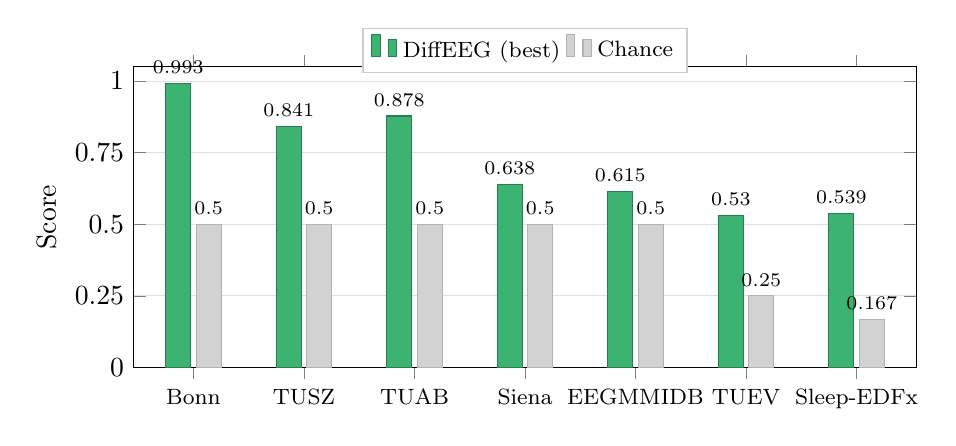
\begin{tikzpicture}
\begin{axis}[
  ybar,
  width=0.95\textwidth, height=5.4cm,
  bar width=9pt,
  enlarge x limits=0.09,
  ymin=0, ymax=1.05,
  ytick={0,0.25,0.5,0.75,1.0},
  ymajorgrids, grid style={gray!25},
  ylabel={Score},
  symbolic x coords={Bonn,TUSZ,TUAB,Siena,EEGMMIDB,TUEV,Sleep-EDFx},
  xtick=data,
  xticklabel style={font=\footnotesize},
  legend style={at={(0.5,1.13)}, anchor=north, legend columns=2, font=\footnotesize, draw=gray!40},
  nodes near coords, nodes near coords style={font=\scriptsize},
  every node near coord/.append style={/pgf/number format/fixed, /pgf/number format/precision=3},
]
\addplot[fill=barB, draw=barB!70!black] coordinates
  {(Bonn,0.993) (TUSZ,0.841) (TUAB,0.878) (Siena,0.638) (EEGMMIDB,0.615) (TUEV,0.530) (Sleep-EDFx,0.539)};
\addplot[fill=gray!35, draw=gray!60] coordinates
  {(Bonn,0.5) (TUSZ,0.5) (TUAB,0.5) (Siena,0.5) (EEGMMIDB,0.5) (TUEV,0.25) (Sleep-EDFx,0.167)};
\legend{DiffEEG (best), Chance}
\end{axis}
\end{tikzpicture}
\caption{Best DiffEEG score per dataset versus chance level. Metric per dataset:
ROC-AUC for Bonn, TUSZ, and TUAB; macro-F1 for Siena and TUEV; accuracy for
EEGMMIDB (2-class) and Sleep-EDFx (6-class). Every task exceeds its chance
baseline, from strong seizure/abnormality transfer to above-chance motor imagery
and sleep staging.}
\label{fig:transfer}
\end{figure*}

Each dataset is reported in its own table listing every adaptation regime we
evaluated---trained head only (frozen backbone), and fine-tuning with the
backbone unfrozen, each with and without the RL head. Bold marks the
best-accuracy row; ``--'' denotes a configuration that was not run. Binary
scores are reported at the F1-optimal operating point (threshold tuned on the
validation set); ROC-AUC and PR-AUC are threshold-free.

\subsection{Seizure detection: TUSZ, Siena, Bonn}
On the official patient-wise TUSZ evaluation split (\num{228667} segments,
$6.7\%$ ictal prevalence, Table~\ref{tab:tusz}), the trained head already
reaches accuracy \num{0.908} and ROC-AUC \num{0.850}. Unfreezing the backbone
with the RL head gives the best operating point overall: accuracy \num{0.940},
macro-F1 \num{0.732}, seizure-F1 \num{0.496}, ROC-AUC \num{0.841}, and PR-AUC
\num{0.484}---a substantial gain in sensitivity to the rare ictal class. A
four-class seizure-subtype task under strict patient-wise cross-validation
additionally reaches macro-F1 $0.363\pm0.020$, with common subtypes separating
well and rare subtypes remaining difficult.

\begin{table}[t]
\centering
\caption{TUSZ seizure detection (patient-wise evaluation split). Sz-F1 $=$
seizure-class F1.}
\label{tab:tusz}
\scriptsize
\setlength{\tabcolsep}{3pt}
\begin{tabular}{@{}lccccc@{}}
\toprule
Adaptation & Acc & Macro-F1 & Sz-F1 & ROC-AUC & PR-AUC \\
\midrule
Head only, no RL       & 0.908 & 0.697 & 0.444 & \best{0.850} & 0.429 \\
Head only, $+$RL       & 0.911 & 0.689 & 0.426 & 0.836 & 0.369 \\
Unfrozen, no RL        & \multicolumn{5}{c}{-- (not run) --} \\
\textbf{Unfrozen, $+$RL} & \best{0.940} & \best{0.732} & \best{0.496} & 0.841 & \best{0.484} \\
\bottomrule
\end{tabular}
\end{table}

Siena is an extreme-imbalance benchmark ($0.64\%$ ictal prevalence,
Table~\ref{tab:siena}). A frozen trained head reaches accuracy \num{0.951} and
macro-F1 \num{0.528} but calls many false positives (seizure precision
\num{0.046}). Full fine-tuning with the RL head raises accuracy to \num{0.992}
and macro-F1 to \num{0.638}, lifting seizure precision roughly eight-fold (to
\num{0.366}) and reducing false positives by an order of magnitude---a far more
usable operating point for continuous monitoring. Zero-shot reuse of the TUSZ
head is unusable here (ROC-AUC \num{0.626}, tens of thousands of false
positives).

\begin{table}[t]
\centering
\caption{Siena seizure detection ($0.64\%$ ictal prevalence). Sz-P $=$ seizure
precision.}
\label{tab:siena}
\scriptsize
\setlength{\tabcolsep}{3pt}
\begin{tabular}{@{}lccccc@{}}
\toprule
Adaptation & Acc & Macro-F1 & Sz-F1 & Sz-P & ROC-AUC \\
\midrule
Head only, no RL       & 0.951 & 0.528 & 0.080 & 0.046 & 0.734 \\
Head only, $+$RL       & \multicolumn{5}{c}{-- (not run) --} \\
Unfrozen, no RL        & \multicolumn{5}{c}{-- (not run) --} \\
\textbf{Unfrozen, $+$RL} & \best{0.992} & \best{0.638} & \best{0.280} & \best{0.366} & -- \\
\bottomrule
\end{tabular}
\end{table}

Bonn is a small curated seizure/normal benchmark in which each record provides a
single trace placed in one of the $22$ channels (Table~\ref{tab:bonn}). Even so,
the trained head reaches ROC-AUC \num{0.993}, PR-AUC \num{0.974}, and accuracy
\num{0.930}; zero-shot reuse of the TUSZ head already gives ROC-AUC \num{0.716}.
Seizure morphology is thus strongly captured even from minimal spatial coverage.

\begin{table}[t]
\centering
\caption{Bonn seizure vs.\ normal (single active channel).}
\label{tab:bonn}
\scriptsize
\setlength{\tabcolsep}{3pt}
\begin{tabular}{@{}lccccc@{}}
\toprule
Adaptation & Acc & Macro-F1 & W-F1 & ROC-AUC & PR-AUC \\
\midrule
Zero-shot              & 0.846 & 0.643 & -- & 0.716 & 0.647 \\
\textbf{Head only, no RL} & \best{0.930} & \best{0.903} & \best{0.934} & \best{0.993} & \best{0.974} \\
Unfrozen               & \multicolumn{5}{c}{-- (not run) --} \\
\bottomrule
\end{tabular}
\end{table}

\subsection{EEG abnormality and events: TUAB, TUEV}
On the roughly balanced TUAB abnormality-detection task
(Table~\ref{tab:tuab}), a frozen trained head reaches accuracy \num{0.645} and
ROC-AUC \num{0.776}. Unfreezing the backbone improves this markedly: the
best-accuracy configuration reaches accuracy \num{0.793}, F1 \num{0.771}, ROC-AUC
\num{0.878}, and PR-AUC \num{0.877}.

\begin{table}[t]
\centering
\caption{TUAB abnormality detection (balanced binary). $n$ $=$ number of
unfrozen downsampling blocks; Sens/Spec $=$ sensitivity/specificity.}
\label{tab:tuab}
\scriptsize
\setlength{\tabcolsep}{3pt}
\begin{tabular}{@{}lcccccc@{}}
\toprule
Adaptation & Acc & F1 & Sens & Spec & ROC-AUC & PR-AUC \\
\midrule
Head only, no RL         & 0.645 & 0.690 & 0.855 & 0.466 & 0.776 & 0.756 \\
\textbf{Unfrozen ($n{=}2$), no RL} & \best{0.793} & 0.771 & 0.753 & 0.828 & \best{0.878} & \best{0.877} \\
Unfrozen ($n{=}3$), no RL & 0.789 & \best{0.772} & 0.776 & 0.800 & 0.862 & 0.854 \\
$+$RL variants           & \multicolumn{6}{c}{-- (not run) --} \\
\bottomrule
\end{tabular}
\end{table}

TUEV is a fine-grained event-classification corpus. The three epileptiform
families (spike/sharp-wave, generalized and periodic epileptiform discharges)
are mutually confused at the model's temporal resolution; the original six-class
task therefore collapses to accuracy \num{0.336}. Merging the three into a single
epileptiform class gives a four-class task (artifact, background,
epileptiform, eye movement) on which full fine-tuning reaches accuracy
\num{0.628} and macro-F1 \num{0.530}, with epileptiform precision \num{0.894}
(Table~\ref{tab:tuev}); adding the RL head is comparable (\num{0.606} /
\num{0.499}). The dominant errors are between the two non-epileptiform background
categories, not on the clinically important epileptiform class.

\begin{table}[t]
\centering
\caption{TUEV event classification. Rows are the four-class merged task unless
marked (6-cl).}
\label{tab:tuev}
\small
\begin{tabular}{@{}lccc@{}}
\toprule
Adaptation & Acc & Macro-F1 & W-F1 \\
\midrule
Head only, no RL              & 0.560 & 0.445 & 0.588 \\
\textbf{Unfrozen, no RL}      & \best{0.628} & \best{0.530} & \best{0.651} \\
Unfrozen, $+$RL               & 0.606 & 0.499 & 0.632 \\
Unfrozen, $+$RL (6-cl)        & 0.336 & 0.321 & 0.347 \\
\bottomrule
\end{tabular}
\end{table}

\subsection{Motor imagery and sleep staging: EEGMMIDB, Sleep-EDFx}
EEGMMIDB is a two-class imagined-movement task (left vs.\ right fist) far outside
the pretraining domain (Table~\ref{tab:mmidb}). The frozen trained head reaches
$53.2\%$ accuracy, and progressively unfreezing the backbone monotonically
improves this to $57.2\%$ and $61.5\%$ (macro-F1 \num{0.615}), well above the
$50\%$ chance. A pooled-random-split diagnostic (mixing subjects) yields a nearly
identical frozen result ($56.9\%$), indicating that the limitation is the
pretraining domain rather than cross-subject transfer.

\begin{table}[t]
\centering
\caption{EEGMMIDB two-class motor imagery (subject-wise split).}
\label{tab:mmidb}
\scriptsize
\setlength{\tabcolsep}{3pt}
\begin{tabular}{@{}lcccc@{}}
\toprule
Adaptation & Acc & Macro-F1 & W-F1 & ROC-AUC \\
\midrule
Head only, no RL                & 0.532 & 0.521 & 0.523 & 0.586 \\
Unfrozen (last level), no RL    & 0.572 & 0.572 & 0.572 & -- \\
\textbf{Unfrozen (all), no RL}  & \best{0.615} & \best{0.615} & \best{0.615} & -- \\
$+$RL variants                  & \multicolumn{4}{c}{-- (not run) --} \\
\bottomrule
\end{tabular}
\end{table}

Sleep-EDFx is a six-class staging task in which only two bipolar EEG channels are
available (Table~\ref{tab:sleep}). Despite this minimal spatial coverage, the
embedding reaches $53.9\%$ accuracy and macro-F1 \num{0.539}, far above the
$16.7\%$ chance. Per class, wake and deep sleep (N4) separate best (F1
\num{0.831} and \num{0.683}), while the light-sleep transitions N1/N2 are the
weakest (F1 \num{0.418}/\num{0.353}), matching their known difficulty for human
scorers. RL adds little here because the task is class-balanced by design.

\begin{table}[t]
\centering
\caption{Sleep-EDFx six-class sleep staging (two bipolar channels).}
\label{tab:sleep}
\small
\begin{tabular}{@{}lccc@{}}
\toprule
Adaptation & Acc & Macro-F1 & W-F1 \\
\midrule
Head only, no RL          & 0.535 & 0.530 & 0.530 \\
Unfrozen, no RL           & 0.535 & 0.538 & 0.538 \\
\textbf{Unfrozen, $+$RL}  & \best{0.539} & \best{0.539} & \best{0.539} \\
\bottomrule
\end{tabular}
\end{table}

\subsection{Mental disorder detection: Mumtaz2016}
Mumtaz2016 is a binary major-depressive-disorder (MDD) versus healthy-control
task from $64$ subjects ($34$ MDD, $30$ control) recorded on the $19$-electrode
$10$--$20$ system, which map onto $19$ of our $22$ canonical channels. We use a
subject-independent split (no subject appears in both train and test). To place
our result alongside the published Mumtaz2016 leaderboard, we reprocess the data
following the protocol adopted by CBraMod and
REVE~\cite{wang2024cbramod,elouahidi2025reve}: only the eyes-open and eyes-closed
resting sessions (the P300 TASK session dropped), a \SI{50}{\hertz} notch filter,
a band-pass filter, and a common-average reference. We keep the backbone's native
\SI{256}{\hertz} (their pipeline resamples to \SI{200}{\hertz}) and use a
$0.1$--$30$~\si{\hertz} band. For contrast we also report our default referential
setup, which additionally includes the TASK session and applies no band-pass.

The preprocessing choice dominates the result (Table~\ref{tab:mumtaz}). Under the
matched pipeline a frozen trained head reaches balanced accuracy \num{0.812},
ROC-AUC \num{0.935}, and PR-AUC \num{0.942}---a \num{0.10} ROC-AUC gain over our
default referential preprocessing (\num{0.832}), recovered almost entirely by the
average reference and band-pass. Notably, under the matched pipeline the frozen
head is the strongest configuration: full fine-tuning lowers balanced accuracy to
\num{0.767}, overfitting the small ($\approx\!\num{5600}$-window) training set---
consistent with the linear-probe strength reported for other EEG foundation
models. Our best balanced accuracy (\num{0.812}) remains below the leaderboard
(EEGNet \num{0.923}, CBraMod \num{0.956}, REVE-Base \num{0.964}), but the AUC
metrics (ROC-AUC \num{0.935}, PR-AUC \num{0.942}) approach the strongest
task-specific baseline (EEGNet AUROC \num{0.964}); the balanced-accuracy gap is
partly a decision-threshold effect, as the frozen head is MDD-biased at the
default threshold (control recall \num{0.66} versus MDD \num{0.96}).

\begin{table}[t]
\centering
\caption{Mumtaz2016 MDD detection (binary, subject-independent split). Two
preprocessing setups: our default referential montage (EC$+$EO$+$TASK, no
band-pass) and the CBraMod/REVE-matched pipeline (EC$+$EO only, \SI{50}{\hertz}
notch, band-pass, common-average reference). Bal-Acc $=$ balanced accuracy;
ROC-AUC/PR-AUC are reported for the frozen-head runs.}
\label{tab:mumtaz}
\scriptsize
\setlength{\tabcolsep}{3pt}
\begin{tabular}{@{}lcccc@{}}
\toprule
Adaptation & Bal-Acc & Macro-F1 & ROC-AUC & PR-AUC \\
\midrule
\multicolumn{5}{@{}l}{\emph{Default preprocessing (EC$+$EO$+$TASK, referential)}}\\
Head only, no RL         & 0.756 & 0.758 & 0.832 & 0.811 \\
Unfrozen, no RL          & 0.768 & 0.769 & -- & -- \\
Unfrozen, $+$RL          & 0.763 & 0.764 & -- & -- \\
\midrule
\multicolumn{5}{@{}l}{\emph{CBraMod/REVE-matched (EC$+$EO, notch $+$ band-pass $+$ avg-ref)}}\\
\textbf{Head only, no RL} & \best{0.812} & \best{0.818} & \best{0.935} & \best{0.942} \\
Unfrozen, no RL          & 0.767 & 0.770 & -- & -- \\
Unfrozen, $+$RL          & 0.768 & 0.772 & -- & -- \\
\bottomrule
\end{tabular}
\end{table}

\subsection{Linear probing: the frozen embedding across tasks}
Table~\ref{tab:linprobe} consolidates the linear-probing result---the frozen
DiffEEG embedding with only a trained classifier head and no backbone
fine-tuning---across all eight downstream datasets, next to the best score
reached anywhere in the adaptation ladder. The probe classifier is the
lightweight two-layer MLP head described in Section~\ref{subsec:headonly}
($4800\!\to\!512\!\to\!256\!\to\!K$, with batch normalization, GELU, and
dropout), trained with class-weighted cross-entropy while every backbone weight
stays frozen; we use ``linear probing'' in the common sense of fitting only a
small head on top of the fixed representation. As a stricter, parameter-free
alternative we also evaluate the same frozen embedding with a
$k$-nearest-neighbor classifier (Section~\ref{subsec:embonly})---a classifier
with no trained weights at all (Table~\ref{tab:knn}). The frozen embedding alone
is already
highly discriminative for morphology-driven clinical tasks: without touching the
backbone it reaches ROC-AUC \num{0.993} (Bonn), \num{0.935} (Mumtaz MDD), and
\num{0.850} (TUSZ), and on TUSZ, Mumtaz, and Bonn the frozen probe is in fact the
strongest configuration. Fine-tuning helps most where the task is furthest from
the pretraining domain (EEGMMIDB motor imagery $0.532\!\to\!0.615$;
TUAB $0.776\!\to\!0.878$ ROC-AUC) and adds little on the tasks the frozen
embedding already solves.

The parameter-free $k$NN probe (Table~\ref{tab:knn}) sharpens this picture: with
no trained weights at all, the embedding's local neighborhoods already separate
the morphology-driven clinical tasks well above chance---Mumtaz MDD
\num{0.791}, Bonn \num{0.775}, Siena \num{0.615} (chance \num{0.5}), and TUEV
\num{0.328} (chance \num{0.25})---but sit exactly at chance for the out-of-domain
BCI and sleep tasks (EEGMMIDB \num{0.500}, Sleep-EDFx \num{0.167}), which only
become separable once a head is trained or the backbone is fine-tuned. The
pretraining domain is thus imprinted directly on the geometry of the embedding
space. True zero-shot transfer (reusing the TUSZ seizure head with no training at
all) is meaningful only within the seizure family and is reported per dataset
above (Bonn ROC-AUC \num{0.716}; Siena \num{0.626}).

\begin{table}[t]
\centering
\caption{Linear probing across tasks: frozen DiffEEG embedding $+$ trained head
(no backbone fine-tuning). ``Best'' is the top of the full adaptation ladder for
the same metric (Tables~\ref{tab:tusz}--\ref{tab:mumtaz}). Metric: R $=$ ROC-AUC,
mF1 $=$ macro-F1, Acc $=$ accuracy.}
\label{tab:linprobe}
\small
\begin{tabular}{@{}llccc@{}}
\toprule
Dataset & Task & Metric & Linear probe & Best \\
\midrule
Bonn        & Seizure       & R   & \best{0.993} & 0.993 \\
TUSZ        & Seizure       & R   & \best{0.850} & 0.841 \\
Siena       & Seizure       & mF1 & 0.528 & \best{0.638} \\
TUAB        & Abnormality   & R   & 0.776 & \best{0.878} \\
TUEV        & Events (4-cl) & mF1 & 0.445 & \best{0.530} \\
EEGMMIDB    & Motor imagery & Acc & 0.532 & \best{0.615} \\
Sleep-EDFx  & Sleep (6-cl)  & Acc & 0.535 & \best{0.539} \\
Mumtaz2016  & MDD           & R   & \best{0.935} & 0.935 \\
\bottomrule
\end{tabular}
\end{table}

% ---- tab:knn : parameter-free kNN probe (CV balanced accuracy); job 256573/257782 ----
\begin{table}[t]
\centering
\caption{Parameter-free (non-parametric) probe of the frozen
\num{4800}-dimensional DiffEEG embedding: $k$-nearest-neighbor classification
($k{=}10$, distance-weighted), scored by 5-fold cross-validated balanced accuracy
(imbalance-robust). A classifier with no trained weights---it uses the target
labels only as the neighbor bank, and is therefore distinct from true zero-shot
transfer (reusing the TUSZ seizure head, reported per dataset). Chance
$=1/(\text{\# classes})$. TUAB and TUSZ use the patient-wise pipeline and are
evaluated separately.}
\label{tab:knn}
\small
\begin{tabular}{@{}llcc@{}}
\toprule
Dataset & Task & Chance & $k$NN bal-acc \\
\midrule
Bonn        & Seizure (2-cl)   & 0.500 & 0.775 \\
Mumtaz2016  & MDD (2-cl)       & 0.500 & \best{0.791} \\
Siena       & Seizure (2-cl)   & 0.500 & 0.615 \\
TUEV        & Events (4-cl)    & 0.250 & 0.328 \\
EEGMMIDB    & Motor (2-cl)     & 0.500 & 0.500 \\
Sleep-EDFx  & Sleep (6-cl)     & 0.167 & 0.167 \\
\bottomrule
\end{tabular}
\end{table}

% ==================================================================
\section{Model Interpretation and Embedding Analysis}
% ==================================================================
Clinical adoption of automated EEG analysis requires not only accuracy but also
representations that are inspectable and physiologically plausible. We therefore
analyze what the diffusion embedding encodes and which signal
features drive its clinical decisions, using the frozen pretrained backbone and
the finetuned TUEV classifier.

\subsection{The embedding organizes clinical categories}
Fig.~\ref{fig:tsne} shows a two-dimensional t-SNE projection of the
\num{4800}-dimensional embedding. For Bonn (seizure vs.\ normal), the frozen
pretrained embedding, computed with no task training whatsoever, separates the
two classes into clearly distinct regions, and a $k$-nearest-neighbor
classifier on the raw embedding reaches 77.5\% balanced accuracy (chance
$50\%$). This confirms that seizure morphology is captured by pretraining
alone, consistent with the strong head-only result on Bonn
(Table~\ref{tab:bonn}). For Siena, an independent seizure-detection corpus
with extreme class imbalance (Table~\ref{tab:siena}), the frozen embedding
already separates several sub-regions of seizure windows from the normal
majority, and full finetuning with the RL head visibly consolidates the
seizure windows into more coherent clusters, raising $k$NN balanced accuracy
from 61\% to 71\% (chance $50\%$). The embedding is thus not a black box but
an organized feature space in which clinically distinct categories occupy
increasingly distinguishable regions as adaptation proceeds.

\begin{figure*}[t]
\centering
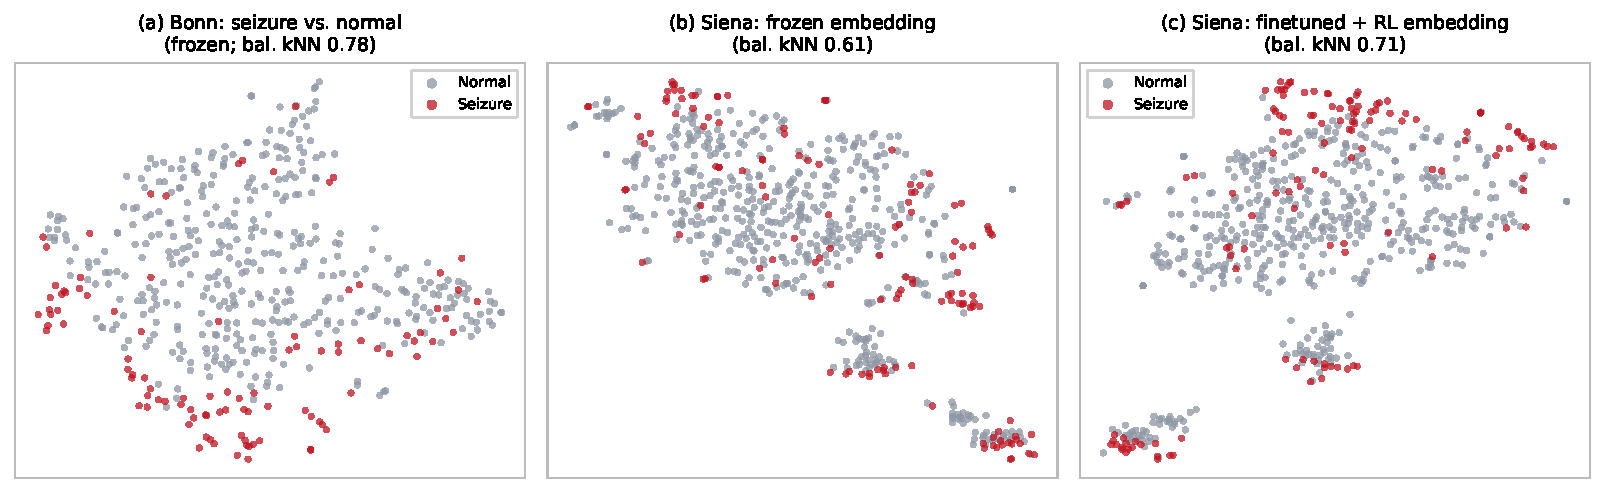
\includegraphics[width=0.98\textwidth]{analysis/fig_tsne.pdf}
\caption{t-SNE of the \num{4800}-dimensional DiffEEG embedding, colored by
class. (a) Bonn seizure vs.\ normal on the frozen pretrained embedding: the
two classes separate without any task training. (b,c) Siena seizure vs.\
normal on the frozen and finetuned+RL embeddings: seizure windows form more
coherent clusters after finetuning. Balanced $k$NN accuracy on the raw
embedding is annotated per panel.}
\label{fig:tsne}
\end{figure*}

\subsection{Saliency localizes the electrophysiology}
To identify which inputs drive a decision, we compute gradient-based saliency for
the epileptiform class---the mean absolute gradient of the epileptiform logit with
respect to the input, averaged over all epileptiform test windows
(Fig.~\ref{fig:saliency}). The resulting scalp map is dominated by
temporal and frontotemporal electrodes (T4, F7, F3, T5) together with
frontal FP2, which matches the well-established temporal-lobe predominance of
interictal epileptiform discharges; occipital and midline-central channels
contribute least. The temporal saliency profile is distributed across the entire
\SI{5}{\second} window with transient peaks rather than being concentrated at a
single instant, consistent with the intermittent, sharp-transient nature of
epileptiform activity. Because the saliency is expressed directly over the
standard 10--20 montage, it can be overlaid on a clinician's electrode map,
providing a physiologically interpretable rationale for each decision.

\begin{figure*}[t]
\centering
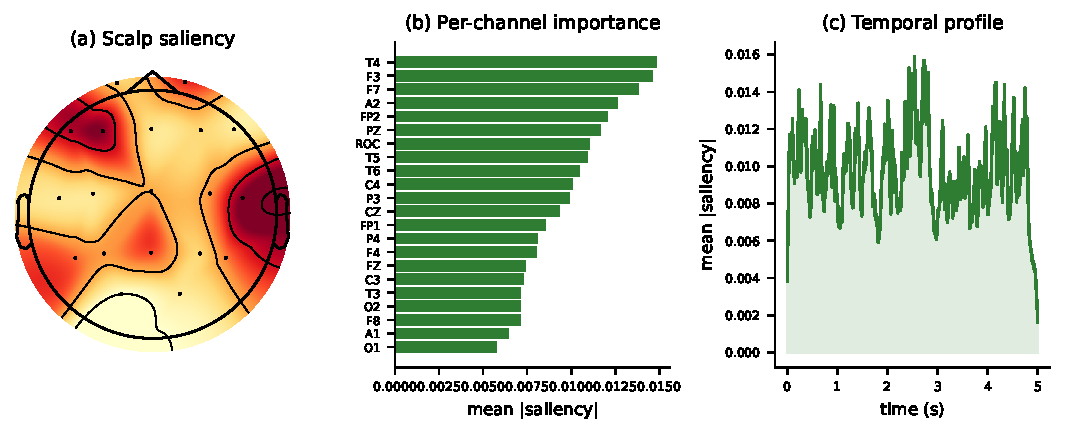
\includegraphics[width=0.98\textwidth]{analysis/fig_saliency.pdf}
\caption{Gradient saliency for the epileptiform class (TUEV). (a) Scalp
topomap of per-channel importance over the 19 mappable 10--20 electrodes; hot
regions are temporal/frontotemporal. (b) Per-channel importance ranking
(all 22 model channels). (c) Temporal saliency profile across the
\SI{5}{\second} window.}
\label{fig:saliency}
\end{figure*}

% ==================================================================
\section{Discussion}
% ==================================================================
The results show that a purely generative diffusion backbone yields a
representation that transfers across four distinct task families from a single
pretraining corpus. Three patterns are worth highlighting.

\paragraph{Transfer tracks task relatedness} Seizure-like tasks transfer best
(Bonn ROC-AUC \num{0.993}; strong minority precision on Siena), which is
expected given seizure-corpus pretraining. Sleep staging transfers moderately
even from two channels, indicating that the encoder captures broadband
oscillatory structure (delta/theta power, spindles) that is not seizure
specific. Motor imagery transfers the least, and a pooled-split diagnostic
(mixing subjects across train and test) barely changes the frozen result,
localizing the bottleneck to the pretraining domain---the backbone has
not learned sensorimotor-rhythm features---rather than to cross-subject
variability.

\paragraph{Metric-aware adaptation matters under extreme imbalance} The RL head
is decisive where the positive class is very rare: on the
\num{0.64}\%-prevalence Siena corpus it lifts minority-class precision roughly
eight-fold, and it yields the best TUSZ operating point. It is negligible where
the classes are balanced (Sleep-EDFx), and---informatively---on the moderately
imbalanced four-class TUEV task plain fine-tuning slightly exceeds it (macro-F1
\num{0.530} versus \num{0.499}). Practitioners should therefore expect a
macro-F1-aware objective to matter most in the rare-positive regime rather than
under mild imbalance, where additional fine-tuning capacity can suffice.

\paragraph{Temporal resolution bounds fine-grained tasks} The \SI{5}{\second}
window with coarse pooling erases the spike-level morphology that separates
epileptiform subtypes; merging the indistinguishable classes recovers a usable
four-class TUEV task. Fine-grained temporal tasks will benefit from shorter
windows or higher-rate probes.

\paragraph{The backbone is anchored to its \SI{5}{\second} pretraining scale}
Because pretraining used a fixed five-second input, the backbone is most
effective near that scale, and window length must be treated as a constraint
rather than a free hyperparameter (Table~\ref{tab:window}). On Sleep-EDFx,
macro-F1 peaks at \SI{5}{\second} (\num{0.539}) and collapses to near-chance at
both \SI{1}{\second} (\num{0.048}) and \SI{20}{\second} (\num{0.060}): the
\num{256}-sample and \num{5120}-sample inputs are far outside the
\num{1280}-sample pretraining regime, so the frozen features degrade. On the
coarser TUAB abnormality task a modest extension to \SI{10}{\second} is tolerated
and even helps slightly (head-only ROC-AUC \num{0.771}$\to$\num{0.776};
full-finetune accuracy \num{0.732}$\to$\num{0.750}), consistent with the
\SI{10}{\second} window used by foundation-model benchmarks. The practical
implication is that this fixed-length U-Net cannot ingest the long
(\SI{30}{\second}) epochs that sleep staging is scored on; matching such
long-context tasks would require patch-based tokenization or a variable-length
positional encoding, as in CBraMod and REVE, rather than a single fixed window.

\begin{table}[t]
\centering
\caption{Window-size sensitivity. The backbone performs best near its
\SI{5}{\second} pretraining length; extreme deviations collapse to near-chance.
Metric: macro-F1 (Sleep-EDFx), head-only ROC-AUC (TUAB). $^{\ast}$TUAB is a
separate controlled reprocessing through our pipeline, so its absolute values
differ from the main TUAB result (Table~\ref{tab:tuab}); the \SI{5}{}--\SI{10}{}
comparison is internally controlled.}
\label{tab:window}
\small
\begin{tabular}{@{}lccccc@{}}
\toprule
Dataset & Metric & \SI{1}{\second} & \SI{5}{\second} & \SI{10}{\second} & \SI{20}{\second} \\
\midrule
Sleep-EDFx    & macro-F1 & 0.048 & \best{0.539} & --    & 0.060 \\
TUAB$^{\ast}$ & ROC-AUC  & --    & 0.771        & \best{0.776} & --    \\
\bottomrule
\end{tabular}
\end{table}

Channel coverage is a further first-order factor: transfer quality broadly
follows the number of real channels, and results on low-coverage datasets (Bonn,
Sleep-EDFx) should be read as evidence of graceful degradation rather than as
clean montage-transfer tests.

\paragraph{Clinical implications} Three properties align with the demands of
clinical deployment. First, the extreme-imbalance behavior on Siena---an
eight-fold precision gain and an order-of-magnitude reduction in false
positives---directly addresses the dominant failure mode of continuous seizure
monitoring, where a high false-alarm rate makes a detector unusable regardless of
its AUROC. Second, the frozen embedding supports rapid, low-label adaptation: a
new site or task can be served by training only a lightweight head on cached
features, without the compute or data needed to retrain a foundation model.
Third, the saliency and embedding analyses provide a physiologically plausible,
inspectable rationale for each decision (Figs.~\ref{fig:tsne},
\ref{fig:saliency}), which is a prerequisite for clinical trust and regulatory
review. We emphasize, however, that these results are retrospective and
benchmark-based; prospective, multi-site validation with clinician-in-the-loop
evaluation remains necessary before any deployment claim.

\paragraph{Limitations} The comparison to foundation models is positional rather
than strictly like-for-like: while all methods use the official patient-disjoint
splits, they differ in montage, sampling rate, and window length, and matching
every confound would require reprocessing under each protocol. Pretraining used a
single corpus (TUSZ) and a fixed montage, so the model has no built-in montage
invariance and relies on the harmonization front end; low channel coverage (Bonn,
Sleep-EDFx) confounds task difficulty with montage transfer. Finally, we evaluate
a single backbone scale, leaving scaling behavior for diffusion EEG embeddings
open.

% ==================================================================
\section{Comparison with State-of-the-Art}
% ==================================================================
Table~\ref{tab:fm} compares \textsc{DiffEEG} with recent EEG foundation models
on three clinical benchmarks with established baselines: TUAB abnormality
detection (accuracy, ROC-AUC, AUC-PR), TUEV event classification (accuracy,
weighted-F1), and Mumtaz2016 MDD detection (balanced accuracy, ROC-AUC, AUC-PR).
Foundation-model numbers are self-reported; the task-specific
baselines did not evaluate on TUAB/TUEV in their original papers, so their
scores are taken from the common EEG-FM benchmark (originated by BIOT and
reproduced by CBraMod/REVE), as detailed in the table footnote.
All methods---including ours---evaluate on the official patient-disjoint
TUAB/TUEV test partitions, so the comparison is fair with respect to
patient-independence. It remains indicative rather than strictly like-for-like
in other respects: the baselines use their own preprocessing (typically
$16$--$20$ bipolar channels at \SI{200}{\hertz}, and, for TUEV, all
$\num{112491}$ fixed-window segments), whereas \textsc{DiffEEG} uses a
$22$-channel referential montage at \SI{256}{\hertz} and an event-windowed
four-class TUEV task.

\begin{table*}[t]
\centering
\caption{Comparison with task-specific and foundation EEG models on TUAB
(abnormality), TUEV (events), and Mumtaz2016 (MDD detection). Values are
balanced accuracy (Acc), ROC-AUC, and AUC-PR for TUAB; balanced accuracy and
weighted-F1 (W-F1) for TUEV; and balanced accuracy (Acc), ROC-AUC, and
AUC-PR for Mumtaz2016. Foundation-model rows are self-reported; the task-specific
baselines did not originally evaluate on these corpora, so their numbers are
taken from the unified EEG-FM benchmark (see footnote). Best per column in bold;
$\underline{\text{underline}}$ marks the best non-foundation baseline.}
\label{tab:fm}
\scriptsize
\setlength{\tabcolsep}{3pt}
\begin{tabular}{@{}lcccccccccc@{}}
\toprule
\multirow{2}{*}{Model} & \multirow{2}{*}{\makecell{Params\\(M)}} &
\multicolumn{3}{c}{TUAB} & \multicolumn{2}{c}{TUEV} & \multicolumn{3}{c}{Mumtaz2016} \\
\cmidrule(lr){3-5}\cmidrule(lr){6-7}\cmidrule(lr){8-10}
 & & Acc & ROC-AUC & AUC-PR & Acc & W-F1 & Acc & ROC-AUC & AUC-PR \\
\midrule
\multicolumn{10}{@{}l}{Task-specific (non-foundation)}\\
EEGNet~\cite{lawhern2018eegnet}        & 0.003 & 0.764 & 0.841 & 0.830 & 0.388 & 0.654 & 0.923 & 0.964 & 0.963 \\
EEGConformer~\cite{song2022conformer}  & 0.55  & 0.776 & 0.845 & 0.843 & 0.407 & 0.698 & 0.931 & 0.970 & 0.968 \\
SPaRCNet~\cite{jing2023sparcnet}       & 0.79  & 0.790 & 0.868 & 0.841 & 0.416 & \underline{0.702} & \underline{0.932} & \underline{0.978} & 0.975 \\
ContraWR~\cite{yang2021contrawr}       & 1.6   & 0.775 & 0.846 & 0.842 & \underline{0.438} & 0.689 & 0.920 & 0.962 & 0.959 \\
CNN-Transformer~\cite{peh2022cnntrans} & 3.2   & 0.778 & 0.846 & 0.843 & 0.409 & 0.685 & 0.931 & 0.974 & \underline{0.976} \\
FFCL~\cite{li2022ffcl}                 & 2.4   & 0.785 & 0.857 & 0.845 & 0.398 & 0.678 & 0.931 & 0.975 & 0.972 \\
ST-Transformer~\cite{song2021sttrans}  & 3.5   & \underline{0.797} & \underline{0.871} & \underline{0.852} & 0.398 & 0.682 & 0.914 & 0.959 & 0.958 \\
\midrule
\multicolumn{10}{@{}l}{Foundation models}\\
BIOT~\cite{yang2024biot}            & 3.3  & 0.796 & 0.881 & 0.879 & 0.528 & 0.749 & 0.936 & 0.976 & 0.974 \\
EEGPT~\cite{wang2024eegpt}          & 25.0 & 0.798 & 0.872 & -- & 0.623 & -- & -- & -- & -- \\
LaBraM-Base~\cite{jiang2024labram}  & 5.8  & 0.814 & 0.902 & 0.897 & 0.641 & 0.831 & 0.941 & 0.978 & 0.980 \\
CBraMod~\cite{wang2024cbramod}      & 4.2  & 0.829 & 0.923 & 0.926 & 0.667 & 0.834 & 0.956 & 0.992 & 0.992 \\
NeurIPT~\cite{fang2025neuript}      & 73.5 & 0.829 & 0.895 & 0.904 & \best{0.676} & -- & -- & -- & -- \\
REVE-Base~\cite{elouahidi2025reve}  & 69   & \best{0.832} & \best{0.925} & \best{0.928} & \best{0.676} & \best{0.845} & \best{0.964} & \best{0.996} & \best{0.996} \\
BioSerenity-E1~\cite{bettinardi2025bioserenity} & 11.7 & 0.823 & 0.890 & 0.910 & -- & -- & -- & -- & -- \\
\midrule
\textbf{DiffEEG (ours)} & 40.7 & 0.793 & 0.878 & 0.877 & 0.628\textsuperscript{$\dagger$} & 0.651\textsuperscript{$\dagger$} & 0.812\textsuperscript{$\ddagger$} & 0.935\textsuperscript{$\ddagger$} & 0.942\textsuperscript{$\ddagger$} \\
\bottomrule
\end{tabular}
\\[2pt]
{\footnotesize Source of numbers: the task-specific baselines (EEGNet\,--\,ST-Transformer)
did not evaluate on TUAB/TUEV in their original papers; their values are as
re-implemented and reported in the unified EEG-FM benchmark introduced by
BIOT~\cite{yang2024biot} and reproduced by CBraMod~\cite{wang2024cbramod} and
REVE~\cite{elouahidi2025reve} (we cite the REVE appendix tables). The
first-column citations identify the original methods, not the source of
these TUAB/TUEV scores. Foundation-model rows (BIOT\,--\,BioSerenity-E1) and our
own row are self-reported. All methods use the official patient-disjoint
TUAB/TUEV train/test partitions (a single split, with validation drawn from the
training subjects), so every test column is patient-independent; our TUAB uses
the same official split. AUC-PR is a binary metric and is not defined for the
multiclass TUEV task, which is therefore compared on accuracy and weighted-F1
(W-F1). EEGPT does not report TUAB AUC-PR; EEGPT and NeurIPT report TUEV
Cohen's Kappa but not weighted-F1, hence ``--''. The Mumtaz2016 baseline columns
are the balanced-accuracy/AUROC/AUC-PR values from the REVE benchmark (its
Table~9, subject-independent split, all EC$+$EO windows)~\cite{elouahidi2025reve}.
EEGPT, NeurIPT, and BioSerenity-E1 did not evaluate on Mumtaz2016. $\dagger$ Four-class merged,
event-windowed TUEV (macro-F1 \num{0.530}); not directly comparable to the
baselines' six-class setup. $\ddagger$ Frozen-head result under the
CBraMod/REVE-matched preprocessing (EC$+$EO, \SI{50}{\hertz} notch $+$ band-pass
$+$ common-average reference; Table~\ref{tab:mumtaz}).}
\end{table*}

On TUAB abnormality detection, where preprocessing is closest, \textsc{DiffEEG}
attains accuracy \num{0.793}, ROC-AUC \num{0.878}, and AUC-PR \num{0.877}. On
both AUC metrics it surpasses every task-specific (non-foundation)
baseline---the best of which, ST-Transformer, reaches ROC-AUC \num{0.871} and
AUC-PR \num{0.852}---and is on par with the foundation models BIOT and EEGPT,
while remaining below the strongest transformer FMs (LaBraM, CBraMod, REVE at
$0.90$--$0.92$). Models explicitly
designed for montage generalization and trained on far larger corpora
(REVE: \num{60000}\,h / $92$ datasets) lead on cross-montage transfer;
\textsc{DiffEEG} instead shows that a single generative backbone with a
lightweight harmonization front end already transfers usefully across seizure,
abnormality, motor, and sleep tasks at a competitive parameter budget.

On Mumtaz2016 MDD detection, under the matched CBraMod/REVE preprocessing a
frozen \textsc{DiffEEG} head reaches balanced accuracy \num{0.812}, ROC-AUC
\num{0.935}, and AUC-PR \num{0.942}. On these AUC metrics it approaches the strongest
task-specific baselines (e.g.\ SPaRCNet ROC-AUC \num{0.978}) while trailing the
transformer foundation models (CBraMod and REVE at $\ge\!0.99$)---the same
ordering seen on TUAB, and again without any fine-tuning.

\subsection{The effect of test-set class balance}
A subtle but important confound underlies seizure-detection benchmarks.
Foundation-model results on the TUH Seizure corpus are typically reported on a
class-balanced test set, built by keeping seizure-containing records and
undersampling background so that seizures form $\approx\!29\%$ of the windows.
Continuous clinical monitoring, by contrast, is naturally imbalanced: seizures
occupy only $\approx\!6.7\%$ of our patient-wise evaluation split. Because AUPRC
depends strongly on prevalence while AUROC does not, evaluating on a balanced
test set inflates AUPRC and makes a method appear far more precise than it would
be in deployment.

To quantify this, we re-score the identical \textsc{DiffEEG} probabilities
after subsampling the negative class to several target prevalences (200 random
seeds; Table~\ref{tab:prev}). AUROC is invariant ($\approx\!0.836$ frozen,
$\approx\!0.841$ unfrozen) across all constructions, as expected. AUPRC, however,
climbs steeply with prevalence: the unfrozen model rises from \num{0.484} at the
natural $6.7\%$ to \num{0.762} at the $29\%$ construction used by seizure-FM
benchmarks and to \num{0.862} at full balance, with the model completely
unchanged. Evaluated at the same $29\%$ construction as the baselines,
\textsc{DiffEEG} (\num{0.762}) exceeds EEGWNet (\num{0.74}), is on par with
MTP-Virgin (\num{0.78}), and trails the pretraining-heavy BioSerenity-E1
(\num{0.85}). Most of the apparent AUPRC gap is therefore an artifact of test-set
balance rather than of representational quality; the honest, prevalence-invariant
gap is in AUROC ($\approx\!0.84$ vs.\ \num{0.926}), which we attribute partly to
the reference's longer analysis windows (\SI{16}{\second} vs.\ our
\SI{5}{\second}). On the companion TUH abnormality task, the same low-data study
reports AUPRC \num{0.907} (BioSerenity-E1), \num{0.898} (EEGWNet), and \num{0.88}
(MTP-Virgin); \textsc{DiffEEG} reaches \num{0.877} (Table~\ref{tab:tuab}),
competitive with these despite far less pretraining data.

\begin{table}[t]
\centering
\caption{Seizure-detection AUPRC on the TUH Seizure corpus. \textsc{DiffEEG}
probabilities are re-scored at three seizure prevalences (200 seeds); AUROC is
prevalence-invariant, AUPRC rises with the seizure fraction. Baseline models are
as reported in the BioSerenity-E1 low-data study~\cite{bettinardi2025bioserenity}
(best of the fine-tuning-hours curve) at their balanced ($\approx\!29\%$)
evaluation. The $29\%$ \textsc{DiffEEG} row is the matched comparison point.}
\label{tab:prev}
\small
\begin{tabular}{@{}llcc@{}}
\toprule
Model & Test prevalence & AUROC & AUPRC \\
\midrule
\multirow{3}{*}{DiffEEG frozen}   & $6.7\%$ (natural)  & 0.836 & 0.369 \\
                                  & $29\%$ (matched)   & 0.836 & 0.712 \\
                                  & $49\%$ (balanced)  & 0.836 & 0.838 \\
\midrule
\multirow{3}{*}{DiffEEG unfrozen} & $6.7\%$ (natural)  & 0.841 & 0.484 \\
                                  & $29\%$ (matched)   & 0.841 & \best{0.762} \\
                                  & $49\%$ (balanced)  & 0.841 & 0.862 \\
\midrule
EEGWNet~\cite{bettinardi2025bioserenity}        & $\approx\!29\%$ & -- & 0.74 \\
MTP-Virgin~\cite{bettinardi2025bioserenity}     & $\approx\!29\%$ & -- & 0.78 \\
BioSerenity-E1~\cite{bettinardi2025bioserenity} & $\approx\!29\%$ & 0.926 & \best{0.85} \\
\bottomrule
\end{tabular}
\end{table}

% ==================================================================
\section{Conclusion}
% ==================================================================
We presented \textsc{DiffEEG}, a denoising-diffusion foundation model whose
frozen encoder provides a compact, transferable EEG representation. A
multi-timestep diffusion-probing embedding, combined with a channel-
harmonization front end and metric-aware reinforcement-learning adaptation,
transfers across seven datasets and four task families---reaching \num{0.993}
ROC-AUC on Bonn seizure detection, \num{94.0}\% accuracy on TUSZ seizure
detection, \num{0.878} ROC-AUC on TUAB abnormality detection, and above-chance
accuracy on motor imagery and sleep staging that the backbone never encountered
during pretraining. Compared with recent foundation
models, \textsc{DiffEEG} is competitive on clinical abnormality detection while
offering broad, low-cost transfer from a single generative backbone. Future work
will pursue montage-invariant positional encodings and multi-corpus diffusion
pretraining to close the remaining gap to the largest foundation models.

% ==================================================================
\section*{Acknowledgment}
% ==================================================================
The authors acknowledge the Digital Research Alliance of Canada for access to
high-performance computing resources used for the experiments in this study.

% ------------------------------------------------------------------
\begin{thebibliography}{99}
\bibitem{obeid2016tuh} I.~Obeid and J.~Picone, ``The Temple University Hospital EEG data corpus,'' \emph{Front. Neurosci.}, vol.~10, p.~196, 2016.
\bibitem{roy2019dl} Y.~Roy \emph{et al.}, ``Deep learning-based electroencephalography analysis: A systematic review,'' \emph{J.\ Neural Eng.}, vol.~16, no.~5, p.~051001, 2019.
\bibitem{yang2024biot} C.~Yang, M.~B.~Westover, and J.~Sun, ``BIOT: Biosignal transformer for cross-data learning in the wild,'' in \emph{Adv.\ Neural Inf.\ Process.\ Syst.}, vol.~36, 2023.
\bibitem{jiang2024labram} W.-B.~Jiang, L.-M.~Zhao, and B.-L.~Lu, ``Large brain model for learning generic representations with tremendous EEG data in BCI,'' in \emph{Int.\ Conf.\ Learn.\ Represent.}, 2024.
\bibitem{wang2024cbramod} J.~Wang \emph{et al.}, ``CBraMod: A criss-cross brain foundation model for EEG decoding,'' in \emph{Int.\ Conf.\ Learn.\ Represent.}, 2025.
\bibitem{wang2024eegpt} G.~Wang \emph{et al.}, ``EEGPT: Pretrained transformer for universal and reliable representation of EEG signals,'' in \emph{Adv.\ Neural Inf.\ Process.\ Syst.}, vol.~37, 2024.
\bibitem{helwan2025diffeeg} A.~Helwan, L.~Abou-Abbas, H.~El~Amouri, B.~Chikhaoui, and K.~Henni, ``DiffEEG: A self-supervised denoising diffusion model for learning EEG generic representations,'' \emph{IEEE Trans.\ Neural Syst.\ Rehabil.\ Eng.}, 2025 (in press).
\bibitem{ho2020ddpm} J.~Ho, A.~Jain, and P.~Abbeel, ``Denoising diffusion probabilistic models,'' in \emph{Adv.\ Neural Inf.\ Process.\ Syst.}, vol.~33, 2020, pp.~6840--6851.
\bibitem{nichol2021improved} A.~Q.~Nichol and P.~Dhariwal, ``Improved denoising diffusion probabilistic models,'' in \emph{Int.\ Conf.\ Mach.\ Learn.}, 2021, pp.~8162--8171.
\bibitem{perez2018film} E.~Perez, F.~Strub, H.~de~Vries, V.~Dumoulin, and A.~Courville, ``FiLM: Visual reasoning with a general conditioning layer,'' in \emph{AAAI}, 2018.
\bibitem{he2022rl} T.~He \emph{et al.}, ``Reinforcement learning with automated auxiliary loss search,'' in \emph{Adv.\ Neural Inf.\ Process.\ Syst.}, vol.~35, 2022, pp.~1820--1834.
\bibitem{ronneberger2015unet} O.~Ronneberger, P.~Fischer, and T.~Brox, ``U-Net: Convolutional networks for biomedical image segmentation,'' in \emph{Int.\ Conf.\ Med.\ Image Comput.\ Comput.-Assist.\ Interv.}, 2015, pp.~234--241.
\bibitem{fang2025neuript} Z.~Fang \emph{et al.}, ``NeurIPT: Foundation model for neural interfaces,'' in \emph{Adv.\ Neural Inf.\ Process.\ Syst.}, 2025.
\bibitem{elouahidi2025reve} Y.~El~Ouahidi \emph{et al.}, ``REVE: A foundation model for EEG adapting to any setup with large-scale pretraining on 25,000 subjects,'' in \emph{Adv.\ Neural Inf.\ Process.\ Syst.}, 2025.
\bibitem{bettinardi2025bioserenity} R.~G.~Bettinardi, M.~Rahmouni, and U.~Gimenez, ``BioSerenity-E1: A self-supervised EEG model for medical applications,'' \emph{arXiv:2503.10362}, 2025.
\bibitem{lawhern2018eegnet} V.~J.~Lawhern \emph{et al.}, ``EEGNet: A compact convolutional neural network for EEG-based brain--computer interfaces,'' \emph{J.\ Neural Eng.}, vol.~15, no.~5, p.~056013, 2018.
\bibitem{song2022conformer} Y.~Song, Q.~Zheng, B.~Liu, and X.~Gao, ``EEG Conformer: Convolutional transformer for EEG decoding and visualization,'' \emph{IEEE Trans.\ Neural Syst.\ Rehabil.\ Eng.}, vol.~31, pp.~710--719, 2022.
\bibitem{jing2023sparcnet} J.~Jing \emph{et al.}, ``Development of expert-level classification of seizures and rhythmic and periodic patterns during EEG interpretation (SPaRCNet),'' \emph{Neurology}, vol.~100, no.~17, pp.~e1750--e1762, 2023.
\bibitem{yang2021contrawr} C.~Yang, D.~Xiao, M.~B.~Westover, and J.~Sun, ``Self-supervised EEG representation learning for automatic sleep staging (ContraWR),'' \emph{arXiv:2110.15278}, 2021.
\bibitem{peh2022cnntrans} W.~Y.~Peh, Y.~Yao, and J.~Dauwels, ``Transformer convolutional neural networks for automated artifact detection in scalp EEG,'' in \emph{Proc.\ IEEE EMBC}, 2022, pp.~3599--3602.
\bibitem{li2022ffcl} H.~Li, M.~Ding, R.~Zhang, and C.~Xiu, ``Motor imagery EEG classification algorithm based on CNN--LSTM feature fusion network (FFCL),'' \emph{Biomed.\ Signal Process.\ Control}, vol.~72, p.~103342, 2022.
\bibitem{song2021sttrans} Y.~Song, X.~Jia, L.~Yang, and L.~Xie, ``Transformer-based spatial-temporal feature learning for EEG decoding (ST-Transformer),'' \emph{arXiv:2106.11170}, 2021.
\end{thebibliography}

\end{document}
